\documentclass[12pt,letterpaper]{article}
\setlength\textwidth{6in}
\setlength\textheight{9in}
\setlength\oddsidemargin{0.25in}
\setlength\evensidemargin{0.25in}
\setlength\topmargin{-0.0in}
\setlength\headsep{0in}
\setlength\headheight{0in}
\setlength\footskip{0in}
\setlength\parindent{0.0in}
\setlength\parskip{1em}
\pagestyle{empty}
\usepackage{common,epsfig}

\newcommand{\position}{Project Scientist (20111759)}
\newcommand{\lab}{MIT Lincoln Laboratory}
\newcommand{\accro}{MLL}

\newcommand{\statement}{the quality of the research, design, and
  development services of the \lab}

\begin{document}

Lincoln Laboratory\\
Massachusetts Institute of Technology\\
244 Wood Street\\
Lexington, MA 02420-9108

\today

Dear Hiring Professionals:

I am writing you to apply for a position with \lab\ (\accro). In 2002
I earned a B.S. in Physics from the Georgia Institute of Technology
and went on to earn a Ph.D. in Astrophysics from Michigan State
University in 2008. Between the years 2008-2010 I was a university
sponsored postdoctoral fellow at the University of Waterloo in Canada
and currently hold the position of a nationally sponsored postdoctoral
fellow at the Observatoire de la C\^ote d'Azur in France. My unique
education, research, and personal skills are well-matched with
\accro's current teams of research and consulting experts, and I feel
I would be a valued addition that would further improve \statement.

As my curriculum vitae (CV) shows, I have been exceptionally
productive in the research arena for the last 10 years, am proficient
at arriving at publishable results, and have formed numerous fruitful
collaborations. In addition, my research covers a broad-range of
scientific topics and has demanded that I continually refine and
expand my knowledge across multiple disciplines -- an ability I refer
to as ``quickly obtaining a critical mass of knowledge.'' My most
valuable skills, which happen to coincide with the stated objectives
of \accro, are critical thinking, detailed analysis, mathematics,
physics, and dissecting complex problems with the goal of finding
creative/novel solutions. I am extremely organized and goal oriented,
which, when combined with my intellectual capabilities, enables me to
provide positive momentum to any project which I undertake or am
assigned.

My skills are not limited to the scientific or collaborative regimes,
I am also technically proficient and can operate autonomously. My
dissection of a problem thus extends beyond the standard steps of
defining the problem and designing a solution, into implementing and
testing those solutions. In my own work, I focus on a few simple
solution priorities: being straightforward, providing clear
documentation, ensuring extensibility, and modularizing. Then comes
the most enjoyable part: breaking down the solutions and finding ways
to be more creative, which naturally means higher efficiency through
simplicity. It is this process which combines my individual strengths
with those of others on a team, and hence is the nexus of what I
consider the collaborative effort. I feel it is this approach to
problem solving and critical thinking that would make me a valued
asset for \accro.

I have included my CV and am willing to send additional materials as
desired (\eg\ writing samples, personal evaluations, examples of my
technical work). I am interested in further discussing the open
positions with staff of \accro\ and would like the opportunity to
interview, at your convenience. I can be easily reached via the email
address and home phone number provided on my CV. I am an American
citizen by birth, eligible to work in the USA, speak fluent English,
have never been accused (or convicted) of a crime, and am proud of my
impeccable personal history. I thank you for your consideration and
look forward to hearing from you.

Sincerely,\\
\begin{minipage}{7.5in}
\epsfig{file=signature.ps,height=0.75in}
\end{minipage}
Kenneth Cavagnolo\\
117 Northern Ave. Apt. 4\\
Decatur, GA, 30030, USA\\
719-285-9062\\
kencavagnolo@gmail.com
\end{document}
